\documentclass{report}

% need it in .docx form? no problem!
% pandoc -s chapter-1.tex -o chapter-1.docx --bibliography="chapter-1.bib"; mv chapter-1.docx ~/Desktop

\usepackage{import}
\import{../}{gov-style}
% \addbibresource{chapter-1.bib}

\begin{document}
\begin{refsegment}

\section{Introduction}
\subsection{The OPM Attack}
In April 2015, a security engineer named Brendan Saulsbury was performing a routine security upgrade for the US Office of Personnel Management when he noticed some suspicious network activity. From somewhere within OPM, a computer was sending brief updates to a website registered at opmsecurity.org---a domain address designed to look like an official system, but not actually belonging to the US Government or the OPM security team. Saulsbury alerted Curtis Mejeurm, one of OPM's senior IT strategists, and it quickly became clear that this bit of outbound traffic was the surface marker of an iceberg-scale data breach. The US Computer Emergency Readiness Team set up shop the next day in an adjacent basement room and hunkered down to investigate and destroy the malware. 10 days, 2000 items of malware, and 1 scheduled power outage later, government security engineers declared that to the best of their knowledge the threat had been removed.\footcite{koerner_inside_2016} But the work to identify the scope of the damage had only just begun.

Almost immediately, it was publicly speculated that the attack originated from China and had connections to the Chinese government.\footcite{spetalnick_china_2015} Though public-facing officials were reluctant to say so, internal investigators determined that the department had been the victim of an attack perpetrated by an advanced persistent threat (APT), a formally organized and typically state-sponsored group of hackers.\footcite[Attributing a cyberattack is difficult because hackers have endless means to obscure their orgins. In this case, however, the first clue that investigators found was left there on purpose. A particularly effective group of hackers tied to China has made it a calling card of sorts to register sites using the names of members of Marvel's comic book superhero group, The Avengers. In this case, opmsecurity.org was registered under the name "Steve Rogers," better known as Captain America.]{koerner_inside_2016} Initial estimates determined that hackers had stolen the personally identifying information of up to 4 million current and former federal employees, including fingerprint data. They had been present in the system for at least half a year.

Within the first month after the breach was discovered, it became clear that the scope of the attack was well beyond that. The files that the Chinese had obtained included an OPM database of applications for security clearance, which exposed the personal data of not just the applicants but the detailed information they supplied about their family and friends. Millions of social security numbers, job applications, and home addresses were now in the hands of a foreign power.\footcite{nakashima_hacks_2015} As FBI Director James Comey put it, ``If you have my SF 86, you know every place I've lived since I was 18, contact people at those addresses, neighbors at those addresses, all of my family, every place I've traveled outside the United States. Just imagine if you were a foreign intelligence service and you had that data.'' And now they did.

\subsection{The Aftermath}
So what did the full power of the United States Government do in response to this massive affront to its security systems and the privacy of citizens? Absolutely nothing. Not a single publicly announced action was taken by the Obama administration that could be interpreted as a retaliatory measure against the Chinese government for stealing the personally identifying information of 21 million Americans.  In case you think I'm missing something, here is the transcript from a July 3, 2017 press briefing---two years after the OPM hack---in which ABC's Jonathan Karl grills Press Secretary Josh Earnest about the administration's lack of response to the OPM hack in the context of its recently announced sanctions against Russia for the election interference (emphasis mine).\footcite[Transcript adapted from the official White House website.]{earnest_press_2017}\footcite[The full exchange goes on for about 5 minutes, and you can watch the entire video here. It's pretty awkward.]{gill_earnest_2017}

\begin{quote}
KARL: So when the Chinese hacked OPM in 2015 [...] why did the White House do nothing publicly in reaction to that hack, which, in some ways, was even more widespread than what we saw here from the Russians, allegedly?
\newline \newline
EARNEST: Well, I think that what we've seen is that these are two cyber incidents that are malicious in nature, but materially different.
\newline \newline
KARL: Twenty-one million people had their personal data taken.  Fingerprints, social security numbers, background checks -- I mean, this was a far-reaching hack.
\newline \newline
EARNEST: \textbf{I'm not downplaying the significance of it, I'm just saying that it's different than seeking to interfere in the conduct of a U.S. national election.} I can't speak to the steps that have been taken by the United States in response to that Chinese malicious cyber activity.
\end{quote}

But... why? What is it about election interference that demands a material sanction from the US Government that is not true of enormous data theft? Karl doesn't let the Press Secretary off the hook with respect to the severity of the incident, correctly pointing out that the harm to US citizens is comparable. The difference, though Earnest was either not equipped or not interested in saying so, is that in this case the government continuously characterized the OPM attack as a form of traditional espionage---spying to build up a database of information about US officials.\footcite{nakashima_chinese_2015}

That intelligence gathering is its own unique category of cyberattack---meriting a separate set of norms---is not explicitly codified anywhere. Instead, it is a generally understood ``rule of the road'' by the relevant actors on both sides. In the Congressional Research Service report commissioned in the aftermath of the breach, they quote an unnamed Senior Administration Official a saying The White House has been clear ``that there is a vast distinction between intelligence-gathering activities that all countries do and the theft of intellectual property for the benefit of businesses in the country, which we don’t do and we don’t think any country should do.'' The CRS report concludes that as of now, the OPM breach ``appears to be seen in the category of intelligence-gathering, rather than commercial espionage.''\footcite{finklea_cyber_2015} And though he avoided repeating it, James Clapper, director of national intelligence, went so far as to say ``you have to kind of salute the Chinese for what they did,'' explicitly condoning a certain level of interstate espionage and offering a tacit acknowledgment of why further sanctions were not pursued.\footcite{sanger_u.s._2015}

Back to Earnest, who confirms that with 17 days left of the Obama presidency his administration had completely opted against any public retribution:

\begin{quote}
KARL: But nothing was announced. There was not a single step announced by the White House in response to that.
\newline \newline
EARNEST: That is true that there was no public announcement about our response, but I can't speak to what response may have been initiated in private.
\newline \newline
KARL: \textbf{But no diplomats expelled, no compounds shut down, no sanctions imposed, correct?}
\newline \newline
EARNEST: Well, again, I can't speak to --
\newline \newline
KARL: \textbf{You don't do that stuff secretly.}  I mean, that's --
\newline \newline
EARNEST: Well, certainly when it comes to the diplomats, that's right, there were no diplomats PNGed. That's something that we would announce publicly.
\end{quote}

Not only can you not do ``that stuff'' secretly, establishing norms and deterring future malicious behavior generally requires that you do it as publicly as possible. At the time, The White House even acknowledged that they needed to be more public in their response for the purposes of deterrence,\footcite{sanger_u.s._2017} and was said to have been considering covert cyber-measures as well as putative economic sanctions,\footcite{nakashima_hacks_2015} the latter of which never materialized. Obama administration officials refused until the very end to name China, and a September 2018 press conference with National Security Advisor Tom Bolton was the first time a US Government official formally attributed the OPM hack to the Chinese government.\footcite{sanger_trump_2018} By then, the window for a comeback response was long gone.

There are a number of high-profile cyberattacks in recent years to chose from, but the OPM hack best illustrates the central question that motivates this thesis: why does the United States appear to allow a number of highly damaging cyberattacks to happen without meaningful public retribution? The 2018 National Cyber Strategy of the United States of America is undoubtedly correct when it states that ``Russia, Iran, and North Korea conducted reckless cyber attacks that harmed American and international businesses and our allies and partners without paying costs likely to deter future cyber aggression.''\footcite{trump_national_2018} Do we in fact have to take James Clapper at his word, and salute the Chinese for an honest piece of intelligence work? I believe that we do---at least insofar as it helps us to understand why the United States policy response to major federal cyber breaches so often feels disproportionately muted.

Attempting to explain the US response to cyberattacks through international norms is not constructionist fancifulness. It is using the exact same terms that policymakers at the highest levels of government do. With regards to the question of cyber espionage's permissibility, House Intelligence Committee member Adam Schiff (D-Calif.) states with surprising candor that ``We want to draw a bright line” that hacking for economic benefit “is a violation of international norms.''\footcite{nakashima_hacks_2015} Why the United States might, or might not, want to draw the line there is what this thesis hopes to answer.






\section{A brief history of US cyber policy}
\subsection{Development of domestic cyberlaw}
In order to understand how norms develop in the international community, it is first important to understand how the United States has evolved in its definition of cyberattack and associated repercussions for perpetrating one. Absent comprehensive, enforceable treaties,\footnote{There are, of course, \emph{some} treaties that deal with international cyber law. They are however few and far between, and with the possible exception of the Budapest Convention, mostly irrelevant to the decision-making of major actors today. I do not have time to comprehensively address that in this draft the way that I will the domestic law, but I imagine some analysis of the existing norms interplay with the nascent cyber treaties will make its way into this thesis.} there is no separate set of laws that guide the prosecution of domestic and international cyber crimes. There are only the domestic laws, with which we can prosecute domestic criminals or foreign nationals who happen to wander into friendly territory, and whatever ability we have to compel compliance with international norms. As such, an overview of how the federal government has conceived of cyber crime is crucial.

Over the second half of the \nth{20} century, policymakers began the process of defining the nature and consequences of what would come to be called a cyberattack. Computer and network security had been a concern for government officials since computers were first integrated into public offices, but it took a long time before cybersecurity in a broader sense would be recognized as the crucial battlefront that it is today.

Early on, policy recommendations for securing government computers focused on addressing specific types of vulnerabilities, rather than broader strategic concerns. A reasonable place to start in the history of cybersecurity policy is with a General Accounting Office recommendation from 1977 titled ``Security of Computer Systems.''\footcite{washington_post_staff_timeline_2003} Delivering the report in testimony before the Congressional Subcommittee on Consumer Affairs, GAO director Donald Scantlebury warned that Government computer systems were insufficiently prepared to defend against ``actions such as crimes, espionage, mischief, and sabotage.''\footcite{u.s._government_accounting_office_security_1977} In the report, he uses the example of a ``computer burglar'' to illustrate how malicious entities might use computer systems to gain access to confidential information or submit fraudulent requests for payment. After a few attempts, Congress and the Reagan administration passed the first federal computer crime legislation seven years later,\footcite[This later bill, the Computer Security Act of 1987, describes the 1984 bill as being the first federal legislation in this area.]{glickman_computer_1988} the ``Counterfeit Access Device and Computer Fraud and Abuse Act of 1984,'' which made it a federal offense to produce a ``fraudulent access device.''\footcite{hughes_access_1984}

The first recognized computer worm (a type of virus) was unleashed on the early internet by Robert Morris, a Cornell graduate student in 1988, supposedly by accident. The self-replicating virus crashed thousands of computers connected the to government's internet precursor, ARPAnet, before it finally was  contained a few days later.\footcite[This source, a master's thesis for the USAF Air University, makes the dramatic and completely unsubstantiated claim that the Morris worm infected half of of ARPAnet's 88,000 computers. The more popular (and plausible) claim is that of the roughly 60,000 ARPAnet-connected computers, the worm infected 10\% of them, though that number is not particularly well substantiated either.]{moore_conception_2014} A GAO report requested by Congress in the event's aftermath noted that cases like these were still somewhat difficult to prosecute due to the lack of federal statutes directed at computer-virus-type incidents.\footcite{u._s._government_accounting_office_computer_1989} That didn't stop the Justice Department from making an example out of Morris as one of the first felony convictions under the Computer Fraud and Abuse Act. The worm and its aftermath permanently altered the public perception of the internet, which until then had felt ``like a small town where people thought little of leaving their doors unlocked.''\footcite{lee_how_2013}

The relevance of this history to US foreign policy with respect to cybersecurity is twofold. First, it illustrates the continuous development of the legal framework under which the United States government evaluates the harm---and justifies a response---to an abstract domestic cyberattack. As we shall see in a few moments, the application of domestic laws to international practice is one of the ways in which proper use norms for a new technology develop. Secondly, the Morris Worm and dearth of available laws with which to respond to it demonstrates the relative recency of the moment in which the inevitability of a malicious attack on federal computer systems was first taken seriously. Robert Morris was a bored 23 year-old who wanted to see how much of the nascent internet his program could reach and unintentionally demonstrated its massive potential for harm. But while his mistake primed policymakers to consider the danger of such an attack, it also set a precedent for thinking of cyberattacks as a one-off. A terrorist or a teen might seek to infiltrate the Department of Defense, and they ought to be prosecuted in response, but there was no external political implication attached. What that external political implication should be is something that policymakers struggle with to this day.

For the remainder of the \nth{20} century, the Federal Government stepped up its focus on securing ``critical infrastructure,'' in which the internet was now see as both a critical target itself and a vector for attacks on others. The George H.W. Bush White House because the first administration to issue a directive treating network security as a pressing national security issue. The official objective of National Security Directive 42 was, perhaps a bit redundantly, ``Ensuring the security of national security systems.'' The government was waking up to the sheer extent to which their critical infrastructure was vulnerable to a cyberattack\footcite{bush_national_1990}, but NSD-42 does not actually address the likelihood of, much less the proper method of responding to, an attack originating from a hostile foreign power.

Between 1992 and 2000, the internet and its potential for commerce and society became abundantly clear to American society. President Clinton firmly integrated cybersecurity into the broader strategic planning of national security and defense, even if it wasn't quite clear at the time what they were protecting and how they were to do it. In September 1993, he issued Executive Order 12864, which established the Council on the National Information Infrastructure. The definition of a National Information Infrastructure is left rather vague, but it essentially describes the public structure that would come to be known as the World Wide Web: ``hardware, software and skills that will make it easy and affordable to connect people with each other, with computers, and with a vast array of services and information resources.'' In 1996, Executive Order 13010 created the President's Commission on Critical Infrastructure Protection, designed to protect ``critical infrastructures from physical and cyberthreats and assuring their continued operation.'' In this space, ``Critical Infrastructure'' has a more well-defined meaning, understood to cover utilities like water, power, fuel, telecommunications, and financial services.\footcite[~p.761. Completely omitted from this thesis is the concurrent debate about the role the government should play in regulating encryption technology. At the same time it was drafting the Executive Orders mentioned above, the Clinton administration was also taking executive action to manage encryption. The encryption debate (which is still ongoing today) raises a lot of questions about the relationship between the federal government, civil liberties, and law enforcement, as well as more generic national security concerns. It is however mostly irrelevant the specific international political questions that motivate this inquriy, and as such is not included here.]{boys_clinton_2018} The inclusion of cyberthreats alongside physical ones signifies a landmark understanding of the actual threat that the internet posed---not just as a new system of infrastructure to defend, but as a vector by which all legacy infrastructure was soon to be made vulnerable as well.

In the last few years of the millennium we see the first policy recommendations that recognize the internet could be be used as a means of attack by a hostile foreign power. CIA Director John Deutch testified to the Senate in 1996 that ``hackers, criminal groups, and foreign intelligence services consider [information systems] lucrative targets,'' noting that a handful of foreign nations have already instituted ``formal information warfare programs.''\footcite{deutch_worldwide_1996} In 1998, cybersecurity for the first time merited its own section in the annual National Security Strategy,\footcite[~p.761]{boys_clinton_2018} and in the subsequent strategy released in 1999, the White House warned that cyberattacks ``could originate from terrorists or criminal groups as well as hostile states.'' Policymakers and presidents had finally identified the danger of cyberattacks and their potential as a tool for war, but they still weren't conceiving of cyberspace as a unique domain for international competition, one deserving of its own ``rules of the road.''


\subsection{Translating domestic law into international strategy}
Jump ahead to the present day, and a few international incidents later, it is clear that cyberattacks are one of the dominant ways that states compete with each other in the international system. Starting with the Clinton administration's National Plan for Information Systems Protection, each American presidential administration has put out a document detailing their cyber strategy.\footnote{In order: "The National Plan for Information Systems Protection" (Clinton), "National Strategy to Secure Cyberspace" (Bush), "International Strategy for Cyberspace: Prosperity, Security, and Openness in a Networked World" (Obama), "National Cyber Strategy of the United States of America" (Trump). The Trump strategy bizarrely claims that it is the "first fully articulated cyber strategy in 15 years." It does not specify whether they simply ignored the Obama-era strategy document or if they don't consider it to be a "fully articulated cyber strategy" for some reason, but the statement is in either case incorrect.} These plans tend to be long, heavy on agencies and committees, and not particularly interesting. Most importantly, they are all incredibly vague as to how the United States will respond to a cyberattack by a foreign power.

Because our current cyber strategy builds on the work of statutes, directives, and norms from past administrations, proving that our stated cyber strategy is lacking in response mechanisms requires looking briefly at each one. The Bush strategy was criticized at the time of its release for its supposed toothlessness---it was heavy on the promoting the private sector's responsibility to voluntarily secure their own networks, and introduced no new enforcement mechanisms.\footcite{lemos_bush_2003} Obama introduced quite a few new official directives on the topic of cybersecurity, but for most of his presidency these were short on enforcement mechanisms as well. While assessing Obama's efforts to secure the nation against cyberthreats in 2013, PolitiFact described the release of his cyberstrategy and its associated directives, then bluntly noted ``So that's what has happened. What hasn't happened: a change in law.'' They gave his promise to ``develop a comprehensive cybersecurity and response strategy'' a grade of ``In the Works.''\footcite{moorhead_work_2013}

Despite the controversy surrounding Russian interference in the 2016 election---and President Trump's subsequent reluctance to address or attribute it---so far there really isn't much daylight between his administration's stated strategy on cybersecurity and that of the administration prior. Though more martial and aggressively worded as per his style, Trump's 2018 cybersecurity strategy offers few specifics that contradict any Obama-era strategy. Christopher Painter, the former White House Senior Director for Cyber Policy, argued at the time that it ``sends a strong message of continuity to our public and our partners.''\footcite[Painter also served at the State Department for six years as the Coordinator for Cyber Issues, which at the time was an Assistant Secretary level position. Since then, its status within the department has fluctuated wildly. Rex Tillerson, Trump's first Secretary of State, announced that he would abolish the office and merge it into State's Bureau of Economic Affairs. Then, just a few months later, he proposed creating an entirely new department bureau with a Senate-confirmed Assistant Secretary, possibly in response to criticism of his first decision. Though current Secretary Mike Pompeo appears to have more interest in cyber policy, the State Department still has not reestablished a high level cyber position.]{painter_white_2018} Part of the continuity is because a lot of Obama's achievements in the cyber realm were heavily technocratic, and the ``National Cyber Strategy of the United States of America'' is light on specifics to contradict them.\footcite{guest_blogger_white_2018} Towards the end of his presidency, Obama signed measures to promote public-private information sharing, secure financial transactions, and establish the Cyber Threat Intelligence Integration Center.\footcite[Among other actions taken during the Obama presidency, these were sufficenct for PolitiFact to update its 2013 rating of his promise to ``Promise Kept.'']{carroll_obama_2016} Most of these measures are still on the books, and as far as we know continue to guide our cyber attack response.

Most importantly for the purposes of this topic, The Obama administration outlined countermeasures that acknowledged cyberattacks would happen and avenues for punishment were required. This was a crucial evolution in our understanding cyberattacks as a full-featured weapon of diplomacy and war, and its one that the Trump administration has embraced. Early cybersecurity strategies focused heavily on defense and prevention, but it the years since it had become clear that cybersecurity policy was as much in need of strategies for mitigation and response. Just as the military would never say that its "missiles strategy" was to not get hit by missiles, so too was it time to stop saying that our cybersecurity strategy was to secure our nation against cyberattacks.

There are two Obama-era actions in particular that directly influence our response to cyberattacks today. The first is Executive Order 13694, which authorizes the Secretary of the Treasury ``to impose sanctions on those individuals and entities that he determines to be responsible for or complicit in malicious cyber-enabled activities that are reasonably likely to result in, or have materially contributed to, a significant threat to the national security, foreign policy, economic health, or financial stability'' of the US,\footcite{daniel_our_2015} and it was later amended to include election interference. Not only did the Trump administration leave the order in place, they quietly extended it in 2017.\footcite{uchill_white_2017} The other is Presidential Policy Directive 41, a plan codifying how the federal government rates the severity of a given cyber incident (Figure \ref{severity-schema}), and sets the architecture and principles that guide its response.

\begin{figure}
\centering
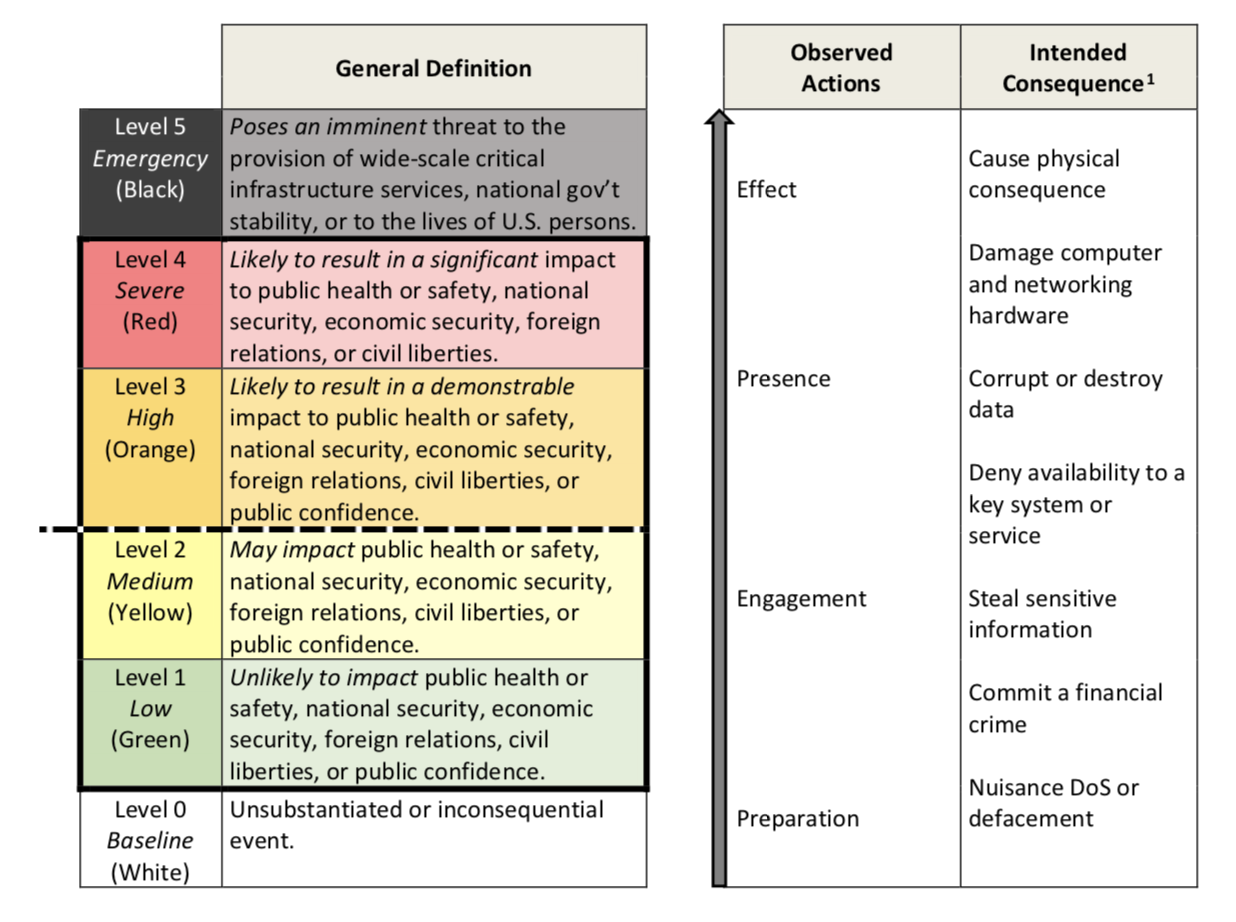
\includegraphics[scale=0.53]{severity-schema.png}
\caption{Cyber Incident Security Schema (The White House 2016)}
\label{severity-schema}
\end{figure}

The one area in which the Trump administration has pointedly diverged from Obama-era cyber policy is in constraints on the offensive use of cyberattacks, and this particular issue is the locus of questions about what sorts of norms the US operates under (and helps to create) when considering cyber operations. In August 2018, President Trump signed a classified order that rescinded Obama's Presidential Policy Directive 20 and had the practical effect of ``delegating authority to the defense secretary to use cyber tools and techniques to disrupt or degrade an adversary's network or choke off attacks underway''\footcite{nakashima_trump_2018} Previously, such an attack would have to have been vetted by the State Department and intelligence agencies, which some within the DoD and Cyber Command found limiting.

Rescinding PPD-20 is a significant step by the Trump administration to reduce the constraints on US Cyberwarfare operations, though at the risk of shooting from the hip and neglecting other broad concerns (diplomatic, legal, economic) that the military might not weigh equally.\footcite{starks_ramifications_2018} It also reduces some of the incentive to cooperate with civilian intelligence services, increasing the risk that the military might decide to operate without sufficient information, and potentially even compromise an existing operation within a civilian agency.\footcite{hawkins_cybersecurity_2018} General Paul Nakasone, director of both the National Security Agency and the United States Cybercommand and the person with whom the authority to launch a cyberattack now rests, had expressed frustration during his Senate confirmation hearing that America's  adversaries attacked us online with little concern for retaliation.\footcite{sanger_trump_2018}

\subsection{So you say we have a strategy---but do we use it?}
Right now the United States Federal Government, its intelligence agencies, and its military have significant leeway to conduct the cyber operations that they believe best serve the interests of the United States of America. Presidential administrations have spent 20 years issuing documents that stress the need to increasing our cyber defenses, and the past 5 years issuing documents that promise the United States will respond accordingly to a cyberattack that is ``likely to result in demonstrable harm to the national security interests, foreign relations, or economy of the United States or to the public confidence, civil liberties, or public health and safety of the American people.''\footcite{office_of_the_press_secretary_fact_2016}

And yet it remains deeply unclear exactly \emph{what actions} the United States takes to respond to a cyberattack once it has determined the origin and the nature of the harm. How does the color-coded severity chart correspond with the relative severity of retaliatory options, like counterespionage or economic sanctions? How could a severity ranking possibly mesh with the US's supposed interest in tacitly permitting cyber operations that look like they are for the purpose of more classical forms of espionage? The federal government is naturally vague about how it weighs its ``assessment of the risks posed to an entity, national security interests, foreign relations, or economy of the United States or to the public confidence, civil liberties, or public health and safety of the American people,''\footcite{office_of_the_press_secretary_fact_2016} but that vagueness renders the response framework toothless to the point of absurdity.

The OPM hack, for instance, would fall under a Level 2 severity: ``Steal sensitive information.'' But it isn't all that different from the Sony hack of 2014, in which hackers affiliated with the North Korean government leaked enormous amounts of sensitive information from Sony executives, supposedly in retaliation for the upcoming James Franco/Seth Rogen comedy about assassinating North Korean leader Kim Jong-Un.\footcite{barnes_sony_2017} The Sony hack became the first time a sitting US president came out and publicly accused a foreign nation of launching a cyberattack while promising retaliation.\footcite{sanger_u.s._2017} The US actually made good on its threat, and direct sanctions came to North Korea the following year.\footcite{lederman_us_2015}

The key difference between the two hacks is that one was carried out against the US government, and the other was an attempt to embarrass and intimidate a private company. The Cyber Security Severity Index doesn't make that distinction clear---but President Obama did. ``We cannot have a society in which some dictators someplace can start imposing censorship here in the United States.''\footcite{perez_obama_2014} Again, administration officials formally acknowledged the crucial role that norms play in guiding international behavior in the cyber realm. ``These lawless acts of intimidation demonstrate North Korea's flagrant disregard for international norms,''\footcite{perez_obama_2014} said Secretary of State John Kerry. Here, the cyber strategy is no help to us in clarifying what about the Sony hack is violates international norms while the OPM hack is permissible,\footnote{There is a small caveat to this that I will probably expand upon in a later draft: the Sony hack actually did cause some physical damage to Sony's networks, which the government took seriously into consideration when considering their response. That having been said, the public emphasis was on the fact that because the hack was a ``freedom of expression'' issue, it merited such a forceful response from the United States Government.} but an understanding of US norms and values is. Only one of these incidents was seen by decisionmakers as analogous to a traditional form of espionage.

There is probably a way to read the cyber strategy documents outlined in this section such that the public responses to both the Chinese OPM hack and the North Korean Sony hack are internally consistent with stated US strategy. But were such a reading even possible, it would have to be a retroactive justification. There would be no way to come up with the solution to the response simply by looking at the input we are given. The missing variable in this equation is the emerging norms about cybersecurity---the train tracks that the US government is laying down in front of them while simultaneously riding the locomotive.\footnote{For visual context, Google "Wallace and Gromit train tracks gif"} This is what President Obama is referring to in his oft-mentioned bit about taming the ``Wild West'' of cybersecurity: absent treaties and international laws, we have only a brief history of norms to guide us, and each decision carries outsized significance in redefining them.\footcite{sanger_u.s._2017}

Are the norms under which we operate a series of conscious decisions in line with the best security, deterrence, and intelligence practices---or are they an outdated port of Cold War espionage norms that see a distinction between types of security breaches were none exists? If we can use the norms of traditional espionage to understand how we evaluate the harm of cybersecurity failures, then what constitutes ``intelligence-gathering activities that all countries do,'' and what norms guide their acceptability? In determining what the international community does or does not consider acceptable in the context of espionage, we can shed light on what the United States intelligence community would consider acceptable in the world of cyber espionage.





\section{Attempts to answer this question}
\subsection{Cyber norms without espionage}
There is an existing base of literature that attempts to define, or even construct, the norms of cybersecurity out of whole cloth. This approach has its strengths, in particular that it draws upon the existing theoretical literature about international relations norms. Constructivist literature about IR norms is robust and contains important insights about how norms develop in unprecedented situations like the sudden emergence of information warfare. Later on, this thesis will define norms along the lines of this literature base, focusing in particular on ``regulative norms that prescribe, proscribe, and order'' state behavior,\footcite{bjorkdahl_norms_2002} often also called ``the rules of the road.''

The problem with this literature base is that is also tends to be rather generic. It is certainly helpful to understand how states like the US are putting pressure on the international system to implement stricter norms to cyberspace, in the absence of a strong legal framework.\footcite[~p.7]{finnemore_constructing_2016} Likewise noting the lack of strong enforcement mechanisms as a barrier to the formation of norms today helps explain why leaders describe cybersecurity as ``The Wild West''.\footcite{iasiello_what_2016} But while these theoretical underpinnings help bolster the argument that these norms both can regulate state behavior and that states are actively trying to create them, but that doesn't help determine exactly what the norms themselves are.

There are also those who point to existing cases of cyberattacks, analyzed the state's response, and hypothesize that they constitute norms. This is a solid approach, but it works best when the hypothesis is based in a norm that existed prior to the introduction of the internet as a vector for its use. Otherwise, you simply don't have enough cases for it to have any normative force, and the argument is either mostly theoretical\footcite{neutze_cyber_2013} or too specific to be of general use.\footcite{caso_rules_2014} A few articles have actually looked at a particular cybersecurity practice in the context of evolving espionage norms,\footcite{libicki_coming_2017} and attempted to define the ones that they see as emerging, such as the norm against using espionage for private economic gain.\footcite{rascoff_norm_2016} These are the closest to my actual research design---though they don't set out to create a comprehensive framework for state behavior.

\subsection{Espionage through the law}
We can also use older analyses of the role of espionage in interstate competition to shed some light on how cyber espionage is viewed today. As Congressman Schiff put it: ``traditional foreign intelligence activities [...] may look untraditional now that they’re in the cyber realm,'' but they essentially follow the same set of rules.\footcite{nakashima_hacks_2015} Many of the papers that discuss norms in the espionage world actually do so using the legal system as an entry point, even though espionage itself exists in an international legal gray area.\footcite{beim_enforcing_2018} That gray area is precisely why a constructivist analysis of interstate norms is not just useful, but necessary.

While international law does address the topic of intelligence gathering during wartime, it is completely silent on the concept of peacetime espionage.\footcite{radsan_unresolved_2007} Instead, norms around peacetime espionage have typically been analyzed in the context of domestic law.\footcite{demarest_espionage_1995} This is curious, because there are obvious diplomatic considerations that affect how we handle foreign nationals convicted of espionage, yet no international acknowledgment of the practice exists, so informal norms must fill the gap.

And naturally there are those who have attempted to jump straight analyzing the potential for cyberlaw to resolve existing issues. A number of these papers are prescriptive, which this paper fundamentally is not, and they attempt to provide a framework for cyber operations either in a civilian\footcite{yurcik_internet_2001} or military\footcite{kehler_rules_2017} legal context. Some even attempt to place existing norms, like the norm against economic espionage, into the context of international law.\footcite{lotrionte_countering_2015} None, however, have simply set out to define what is or is not permissible in a cyber espionage context, laws or otherwise, and that is what this thesis hopes to do.

\section{Research Design}
\emph{This section is written slightly more informally, acknowledging the work still to be done. It will be later updated with conclusions.}

This thesis seeks to establish the feasibility of evaluating United States cyberattack response through the lens of existing espionage norms. That requires that the thesis be split up into two main sections. The first section will establish what norms were developed by intelligence agencies during the Cold War that might be relevant to cybersecurity today. In it, I will look through examples of Cold War espionage incidents and determine how their risk and response were evaluated by the relevant agencies. While this research will be conducted with an eye towards the way these norms might be in active use today, the argument in this part will simply focus on establishing which norms existed that might be relevant to cyberspace at all.

The Cold War is a richly studied period of American history with clear relevance to today, and at the time of this writing I've just cracked the surface. So far, I've found a some denser anthology\footcite{andrew_secret_2009} books\footcite{johnson_intelligence_2015} that purport to be comprehensive readers on topics in US intelligence. While working on those, I will also be scouring intelligence\footcite{prados_william_2009} histories\footcite{prados_presidents_1996} as well. Armed with a little context on the more obvious intelligence norms we see today, I think I can spot patterns in what sorts of missions and operations were deemed acceptable in the past. There is also the possibility that I come across a more comprehensive compilation of espionage norms, in which case this section of the paper can be dramatically shorter, as it no longer bears the burden to prove these norms by itself.

There is another interesting contemporary source for espionage norms as well. Whenever a spy operation breaks into the mainstream news, publications often seek out subject matter experts to comment on whether the operation as it played out public view is something that fits within existing intelligence norms. This raises two possibilities for my research. The first is simply noting these contemporary spy incidents that have nothing to do with cyber, and if they indicate the presence of a norm. A relevant example that comes up up in both cyber and traditional contexts is the expelling (or PNGing) of diplomats who are known to be agents of foreign intelligence services.\footcite{risen_rules_2001} Though considered a ``rare and provocative action,'' it's one that Obama took in the wake of the 2016 election hacking scandal, in direct continuity with existing practices for responding to especially provocative forms of espionage.\footcite{mazzetti_game_2017} The second possibility is that I could interview a few of these subject matter experts, either in the academic or military realm. Plans for this do not yet exist, but if it happens, it has significant potential benefits. Much of the history of intelligence is inherently oral, and the best way to figure out the rules of the game is to ask someone who knows how to play.

This following section will be to analyze the major cyber attacks that the United States has publicly responded to in the context of traditional espionage norms. There isn't much to say about this until the first part is done. While I'm cognizant of the possibility that espionage norms won't prove to be especially relevant to to cybersecurity norms today, I have seen enough reference to them in the cybersecurity literature and from US officials that I am optimistic that the connection will hold.

\newpage
\printbibliography[heading=subbibliography]

\end{refsegment}
\end{document}
